\documentclass[12pt, letterpaper, ]{article}
\usepackage[style=authoryear, maxnames=2, maxbibnames=99]{biblatex}
\addbibresource{total_biblio.bib}
\addbibresource{datasets.bib}
\usepackage{caption}
\usepackage{geometry}
\usepackage{graphicx}
\usepackage{setspace}
\usepackage{url}
\usepackage{lineno}
\linenumbers
\graphicspath{./images/}
\geometry{
        letterpaper,
        top = 1.27cm,
        bottom = 1.27cm,
        left = 2.54cm,
        right = 2.54cm,
        }
\title{MSc Thesis}
\author{Isaac Peetoom Heida}
\date{December 2022}
\doublespace

\begin{document}

\begin{titlepage}
    \begin{center}
        \vspace*{1cm}

        \textbf{The ecological and genetic drivers of silicon accumulation in cereal crops}

        \vspace{1cm}

        by 

        \vspace{1cm}

        \textbf{Isaac Peetoom Heida}
        
        \vfill

        \textsc{a thesis submitted in partial fulfillment of the requirements for the degree of}

        \vspace{1cm}

        \textsc{master of science}

        in

        \textsc{the faculty of graduate and postdoctoral studies}

        (Plant Science)

        \textsc{the university of british columbia}

        (Vancouver)

        \copyright Isaac Peetoom Heida, 2023
    \end{center}
\end{titlepage}

\tableofcontents

\section{Abstract}

As global agricultural production strains under degrading soil fertility and increasing losses due to climate change, there is growing research interest in new avenues for production improvement. New crop technologies must meet increasing public and regulatory demand for environmental sustainability, encouraging scientists to revisit overlooked or relatively unknown techniques that may unlock productivity gains. One of the promising developments to arise over the past 20 years is the potential of silicon to improve crop plant performance. With benefits to multiple dimensions of crop performance, silicon may be a key tool to guard crop production against uncertain future growing conditions. Our ability to mobilize silicon-based cropping strategies is dependent on a thorough understanding of the ultimate and proximate causes of silicon accumulation, including both the ecological and genetic interactions that can trigger increased uptake. In this thesis, I extend recent advances in our understanding of silicon ecology in cereal crops, testing for the presence of rapid silicification in common canadian crops, as well as using a  genome-wide association study to identify genetic markers associated with high silicon content. 

[to add: results, conclusion]

\section{Lay Summary}

Silicon provides tremendous benefits to plant health, but is not widely utilized in agriculture, despite it being highly abundance and naturally occurring in most soils. One of the main factors limiting it's application in agriculture is our poor understanding of the exact dynamics of how plants absorb and use silicon from the soil. I identified genetic traits associated with high silicon content in \textit{Aegilops tauschii}, a relative of bread wheat, as well as demonstrated that cereal crops (e.g. wheat, barley, oats) have the ability to rapidly uptake silicon from the soil. This rapid uptake means that silicon may be a highly effective defence against insect pests. Combining these results with the genetic data, future research can aim towards creating breeding programs to develop cereal crops that can withstand insect damage based on their silicon content. This development could provide an environmentally friendly strategy to maintain output to feed a growing human population.

\section{Preface}

(This was taken nearly verbatim from Matt's thesis, so need to go back through to make sure I am not plagarizing)

The research presented in this thesis is original and unpublished. Isaac Peetoom Heida and Dr. Juli Carrillo, with assistance from Dr. Jean-Thomas Cornelis, conceptualized and developed the experiment presented in Chapter Two. Isaac Peetoom Heida, Dr. Juli Carrillo and Dr. Gurcharn Singh Brar, with input from Dr. Jean-Thomas Cornelis, conceptualized and developed the experiment presented in Chapter Three.
Isaac Peetoom Heida developed the question and methodology for Chapter Two. Dr. Aaron Beattie, Dr. Mazen Aljarrah, and Dr. Gurcharn Brar provided seeds for the experiment. Isaac Peetoom Heida designed and set up the experiment, processed and analysed the samples, and performed the statistical analysis. Dr. Shaun Barker and the Mineral Deposit Research Unit of the University of British Columbia provided facilities and expertise for the XRF analysis of the tissue samples.
For Chapter Three, Isaac Peetoom Heida led plot set up and maintenance, with assistance from Grace Wang, Vincent Fetterley, Sara Salad, Katherine Buchanan, Martina Clausen, and Paul Fisher, and Matt Tsuruda. Isaac Peetoom Heida led the sample harvest, processing and analysis. Kelly Wang, Grace Wang, and Chelsea Gowton assisted with the sample harvesting. Dr. Daria Reshetniak, Paul Fisher, Lucas Friesen, Katie Pryer, Dr. Kinga Treder, Carly MacGregor, and Grace Wang all provided invaluable assistance with sample preparation. 
Chapters Two and Three of this thesis will be submitted to peer-reviewed journals for publication. For the purposes of this manuscript, actions are depicted in the singular first person. 

\section{Introduction}

\subsection{A case for silicon in agriculture}

As global agricultural production strains under degrading soil fertility and increasing losses due to climate change, researchers are leaving no stone unturned in the search for new technologies for sustainable improvement in crop production. New crop technologies must meet increasing public and regulatory demand for environmental sustainability, encouraging scientists to revisit overlooked or relatively unknown techniques that may unlock productivity gains. Over the past 20 years, plant-silicon relations has emerged as a promising field that may safeguard crop performance and security within a changing biosphere. With benefits to multiple dimensions of crop performance, silicon may be a key tool to guard crop production against uncertain future growing conditions. 

\subsection{Silicon in nature}

Silicon abounds in the earth’s crust, with silicon dioxide (SiO\textsubscript{2}) comprising about 60\% of the crust by mass. Nearly all terrestrial plants grow in soils containing silicon, and thus absorb nominal amounts through passive transport as water is absorbed into the plant. Silicon can be deposited throughout the whole plant, forming amorphous masses of silica, with highly variable geometries (\cite{piperno_phytoliths_2006}). Though widespread benefits of silicon are readily observed in many vascular plant families, the exact mechanism through which silicon acts is still poorly understood (\cite{coskun_controversies_2019}), in part due to the seemingly disparate traits that are promoted under silicon supplementation. When supplemented with silicon, plants are generally more resistant to stress. Silicon supplementation shows efficacy in relieving the negative effects of such abiotic stresses as: soil salinity, soil metal toxicity, cold and heat stress, UV stress, water deficits, and phosphorus deficiencies (\cite{cooke_consistent_2016}). Silicon is also effective at limiting the growth and damage of insect and fungal pests (\cite{fauteux_silicon_2005,massey_herbivore_2007}). Silicon-supplied plants put under stress show transcriptome profiles similar to unstressed plants (\cite{coskun_controversies_2019}). The recently put-forward apoplastic barrier hypothesis suggests that the various benefits gained under silicon supplementation derive from the toughening and sealing action of silicon deposition (\cite{coskun_controversies_2019}). Silicon deposits reduce water loss and radiation/temperature damage, and also limit the spread of effector proteins, dampening the effects of fungal pathogen and herbivore excretions designed to interfere with plant defensive physiology.The toughness of the depositions also serves a more direct mechanical role, as the hardened granules of silicon interrupt the chewing motions of herbivores, wear down mandibles and teeth (\cite{stromberg_functions_2016,waterman_short-term_2021-1}), and reduce the digestive efficiencies of herbivores (\cite{johnson_silicon_2021}). Continuing to untangle the various mechanisms through which silicon delivers beneficial effects to plants is key to fully realizing the potential of silicon in sustainable agriculture. 

\subsection{Silicon in soils and roots}

Plants interact with silicon on a variety of levels, mobilizing it from soil aggregates, transporting it into and throughout their bodies, and finally precipitating it out of their xylem into solid masses in the leaves and stems. Within the soil environment, silicon commonly exists in both crystalline (geologic) and amorphous (biogenic) forms (\cite{haynes_contemporary_2014}). Amorphous silicates can derive from previous plant material that has decayed in the soil, but also from marine and aquatic organisms such as diatoms. Globally, the silicon cycle involves silicates weathering out of terrestrial sediments, moving along water courses, and eventually being deposited in the sea, where it is incorporated into various plankton species, and eventually deposited in seafloor sediments. The continual exodus of silicon from terrestrial sediments over geologic timescales means as ecosystems age, plants become more and more central in the local silicon cycle, with much of the silicon in living plant tissue being recycled from previous plant material decaying in the soil(\cite{de_tombeur_plants_2020}). In highly weathered soils with low nutrient availabilities, plants take a more active role in liberating nutrients, including silicon, for uptake. Organic acids and chelating agents, exuded from plant roots, pry tightly bound nutrients such as phosphorus and silicon from soil aggregates, increasing their availabilities for uptake into the root system (\cite{de_tombeur_silicon_2021-1}). This active scavenging for silicon remains poorly understood, but it may be an important mechanism in plant defence (allowing for increased uptake during a defensive response) and breeding for increased root exudation may improve crop plant performance and nutrient use efficiency (\cite{de_tombeur_silicon_2021}).

\subsection{Silicon transporters}	

One of the most important advances in plant-silicon research was understanding the mechanisms through which silicon is acquired and transported into the plant. Silicon’s most common form in soil solution is silicic acid (H2SiO4), which has a maximum solubility of around 2 mM (\cite{haynes_contemporary_2014}). While there is some evidence that small amounts of silicic acid can be transported during water uptake, this method of transport is insufficient to explain the larger amounts of silicon found in some plant families. Research in rice has identified four proteins that transport silicon into and through the plant body. Two of these proteins (LSi1, LSi2) transport silicic acid from the soil into the roots, while the other two (LSi3, LSi6) act to unload silicic acid from the xylem into leaves and inflorescences (\cite{yamaji_orchestration_2015}). Homologues of these proteins have been identified in other cereal crops, and additional analogous silicon transporter proteins have been discovered in Cucurbitaceae (\cite{reynolds_silicon_2016}). Though not identified, there is a hypothesized fifth protein responsible for loading silicic acid into the xylem (\cite{farooq_silicon_2015}). The expression of these genes, or lack-there-of, can not only influence the total amount of silicon accumulated by the plant, but also its relative distribution, as knockout of LSi6 increases leaf silicon content while decreasing the silicon content of seed husks in rice \cite{yamaji_transporter_2008}. Breeding for silicon content and use-efficiency in crop plants may be crucial to improving crop performance under a changing climate \cite{christian_breeding_2022}. However, we still have a relatively poor understanding surrounding the how genetics influence the silicon phenotype of a plant. Further investigations into how genotypic variation is reflected in the silicon content of plants can aid in the discovery of new genes involved in silicon accumulation, and may provide targets for silicon breeding programs. 

\subsection{Silicon in leaves}	

Once inside the plant, silicon is deposited in specialized silica cells, forming phytoliths (\cite{waterman_short-term_2021}). Silicon deposits show consistent and taxa-specific morphologies, suggesting evolutionary pressure selecting for these bodies to yield certain functions to the plant (\cite{piperno_phytoliths_2006}). In stems, these phytoliths are often long and narrow, oriented parallel with the shoot, and seem to increase structural rigidity(\cite{stromberg_functions_2016}). The use of silicon as a structural component represents a highly energetically efficient strategy, as silicon is ~10x cheaper on an energy unit basis to produce than lignin (\cite{stromberg_functions_2016}). Stem silicification has been investigated as it relates to lodging resistance in cereal crops, and silicon supplementation has been found to reduce the prevalence of lodging in rice and wheat (\cite{dorairaj_influence_2017,muszynska_mechanistic_2021}). In leaves, phytoliths are typically more stout, though they still increase the mechanical toughness of the leaf (\cite{simpson_still_2017}). This overall toughness, and abundance of phytoliths in leaves likely evolved to limit herbivore damage, rather than improve the growth characteristics as in stem phytoliths (\cite{stromberg_functions_2016}). Interestingly, even in the absence of silicon, plants develop silica cells, and rapidly fill them when silicon becomes available (\cite{waterman_short-term_2021-1}). As phytoliths deposit in the leaves, polymerization is aided by interactions with proteins in the cell wall, which control sites of nucleation (\cite{nawaz_phytolith_2019}). Silicon deposition in the leaves can happen on relatively short time scales, outpacing the accumulation of other defensive compounds such as phenolics (\cite{waterman_short-term_2021}). Thus, silicon-based defences in crop plants may be one of the first lines of active anti-herbivore defence, providing rapid and sensitive responses to herbivory. 

\subsection{Looking back and looking forward}

Much of today’s plant silicon work is indebted to the pioneering work of Jones and Handreck (\citeyear{jones_silica_1967}) and the subsequent mapping of silicon across the plant kingdom by Takahashi et al. (\citeyear{takahashi_possibility_1990}). Epstein’s seminal \citeyear{epstein_silicon_1999} paper provided a comprehensive review of the state of knowledge in plant silicon, and has spurred a generation of researchers to extend the preliminary findings of the 20th century out across crop production systems and plant ecologies around the world. Silicon is best studied in the grass family (Poaceae) due to the comparatively high silicon content found in most members of the family (often over 1\% of dry weight), as well as the economic importance of domesticated species within the clade (\cite{reynolds_silicon_2016}). Rice, maize, wheat, and barley alone account for one-third of the worlds’ total cultivated land area (\cite{faostat}), and are all domesticated grass species. Silicon supplementation as an agricultural practice has been extensively studied in rice and sugar cane, as these crops tend to deplete soil silicon stocks, necessitating replenishment by application of silicon-rich amendments (\cite{haynes_contemporary_2014,meena_case_2014}). Due to the overall high silicon content of soils globally, Si is rarely truly limiting in soils, though certain forms of silicon are much more plant available than others (\cite{fraysse_surface_2009}). Thus, the applicability and importance of silicon supplementation is unlikely to be realized in more temperate dry-land production systems, particularly in wheat and barley. This does not however nullify the utility of silicon research in these systems, as great work can still be done to improve the manner and efficiency in which these temperate crops utilize the ample silicon available in their soils. Our ability to integrate silicon as a tool for production improvement in dry-land grain production is currently limited by a poor understanding of the genetic controls over silicon accumulation, as well as a limited understanding about the extent to which dry-land cereals utilize silicon in pest-protection. 

\section{Chapter 1: Identifying rapid silicon accumulation in cereal crops}

\subsection{Introduction}

During times of crisis, having an effective and timely response can limit damage and speed recovery. To address acute damage from herbivores, plants have developed a host of defensive strategies, ranging from changes to the body plan down to the development of novel compounds to poison those that would try to eat the plant (\cite{agrawal_plant_2006}). Due to the vastly different nature and ontogeny of various defensive strategies in plants, plant defences operate across a range of intensities and time scales, from short-term temporary activation, to long-lasting changes in the morphology of the plant (\cite{agrawal_plant_2006, karban_induced_1989}). In most scenarios, induced plant defences are activated in response to an external cue, and build in intensity over time, with defensive hormone signals peaking approximately five hours after the initial induction event (\cite{schmelz_quantitative_2003}). Despite this rapid hormonal response, actual defensive phenotypes are slower to emerge, often operating on the scale of days or generations (\cite{karban_induced_1989}). Many defensive responses are also context dependent, where the identity of the damaging actor, the severity of damage, and a host of other factors interact to determine the final defensive response (\cite{waterman_simulated_2019}). The most effective defensive strategies should be those that can either prevent herbivory outright, or can mount a rapid response to limit damage. These same strategies are also the most promising for crop production, where pest damage represents both an economic and food security cost. Integrating better natural plant defences into crop production systems may be key to reducing the environmental impact of agriculture, but hinges upon a thorough understanding of plant defensive physiology.

One of the most promising avenues for new crop defence is the harnessing of silicon (\cite{reynolds_silicon_2016}). Silicon acts on multiple temporal and physiological scales, delivering broad spectrum resistance to pests, pathogens, and abiotic stressors (\cite{cooke_consistent_2016,coskun_controversies_2019}). Soluble silicon taken up from the soil is deposited predominantly in the leaf epidermis, where it forms solid granules that increase the toughness of the tissue, reducing herbivore digestive efficiency (\cite{cooke_is_2011}). Plant silicon is expressed latently, but also increases in response to herbivory (\cite{takahashi_possibility_1990, }). Multiple studies have demonstrated lasting elevated silicon in response to real and simulated herbivory (\cite{massey_are_2008,hartley_ecology_2016}), and recent evidence points to silicon accumulation as being a relatively rapid response, even preempting some chemical defences (\cite{waterman_short-term_2021}). This rapid action makes silicon accumulation a promising trait for future crop development. Despite the novel results, this pattern has so far been observed in just one species, and only under artificial herbivory via the application of methyl-jasmonate. Though a useful tool for herbivory research, methyl-jasmonate application fails to reproduce a complete herbivory signal for the plant, thus observed changes to plant defence may not be representative of a true herbivory scenario (\cite{strauss_direct_2002}). Testing for this rapid silicon accumulation across a variety of grain crops, and under both simulated (methyl-jasmonate) and real herbivory is a crucial first step towards integrating rapid silicification into our understanding of plant defence and crop protection.

Plant silicon research has mostly focused on members of the grass family (Poaceae) due to their exceptional silicon content within the plant kingdom, as well as the economic importance of domesticated grass species (\cite{reynolds_silicon_2016}). Domesticated crops differ significantly from their wild relatives, due to effects of strong selective pressure imposed by humans (\cite{chen_crop_2015}). Most domesticated crops show much lower genetic diversity than their wild ancestors (\cite{hafeez_creation_2021, smith_domestication_2019}). Initial selection for a few individuals with favourable traits creates a genetic bottleneck, and the majority of allelic diversity is lost. Subsequent selection by humans for agronomically relevant traits can result in concurrent losses of adaptations to natural environments, as the traits that maximize human value (eg. yield, ease of harvest) can come at the cost of ecologically relevant traits such as defence (\cite{whitehead_domestication_2017, chen_crop_2015}). Indeed, in the context of silicon, we can detect clear signals of domestication across the Poaceae family, where wild ancestors consistently have higher baseline silicon content than their domesticated descendants (\cite{simpson_still_2017}). Due to the effects of selection on plant defence it becomes crucial to test new developments in the silicon-defence literature in modern crop species, both to validate their utility towards agricultural production, and to gather further observations on the dynamics of silicon-based defences in the first hours after herbivory.

In this study, I test four globally important cereal crop species for rapid silicon accumulation under artificial and real herbivory. In a glasshouse environment, I grew bread wheat (\textit{Triticum aestivum}), oats (\textit{Avena sativa}), barley (\textit{Hordeum vulgare}) and Triticale ($\times$ \textit{Triticosecale}), and tested the following hypotheses:
\begin{enumerate}
        \item Rapid silicon accumulation is a conserved trait in the Poaceae, and the tested species silicon content would show responses to herbivory consistent with this process.
        \item Due to different phylogeny and domestication history, the tested species would vary in the strength of their silicon accumulation response to herbivory. 
        \item Due to the different cues involved when comparing true herbivory damage and methyl-jasmonate induced defensive induction, the tested species would show different patterns of short-term silicon accumulation in response to cricket (\textit{Acheta domesticus}) herbivory and methyl-jasmonate application. 
\end{enumerate}
This study is a thematic replication of Waterman et al.’s \citedate{waterman_short-term_2021} paper, but attempts to extend the findings to commercially important grain crops. The findings of this study will refine our understanding of the prevalence of rapid silicification in the Poaceae, and will help to inform the value of potential applications of silicon-based defences into grain crops.

\subsection{Methods}

\subsubsection{Plant growth and experimental treatments}

To test the prevalence of rapid silicon accumulation in canadian cereal crops, I selected three cultivars for each of oats, bread wheat, triticale, and barley. Cultivars were selected on the basis of minimizing shared pedigree, and no cultivars shared more than one common ancestor within the last two crossing generations. At the start of the experiment, I germinated seeds in germination trays filled with moist sand. After four days, I transplanted germinated seedlings into 10cm pots filled with SunGro potting mix amended with [amount] of silicic acid. Though potting mix and fresh water contain some amount of plant available silicon, the silicic acid was added to ensure that there would be no silicon limitation to the plants. I randomized the location of each pot within the growing space. The pots were bottom watered on flood tables with nutrient solution. I assigned each plant to one of three herbivory treatments: control, simulated herbivory, or true herbivory. Simulated herbivory was achieved by application of 1 mM MeJA solution to the entire above-ground portion of the plant (Waterman et al. 2021b), while true herbivory was provided by crickets housed in water-pik tubes. Prior to introduction to the the plants, I acclimated crickets by feeding them on the same species used in this trial. Immediately preceding cricket application, I placed them in their tubes and starved them for 24 hours, as this increased the likelihood of the insects initiating feeding rapidly upon exposure to the test plants. 

\subsubsection{Sample harvest and preparation}

24 hours after treatment application, I harvested leaf material by clipping all undamaged (i.e. no cricket exposure) leaves. Leaf tissue was flash frozen in liquid nitrogen, freeze dried, and stored in a -80ºC freezer. To prepare the leaf powder for XRF analysis, I transferred the dried frozen leaf tissue to 2 mL microcentrifuge tube. I then flash froze the tubes in liquid nitrogen and ground the leaf tissue in a tissuelyser bead mill for 30 seconds at 60 Hz.

\subsubsection{Silicon analysis}

To measure the silicon content of the leaf tissue, I followed a modified version of the bench-top XRF method (\cite{reidinger_rapid_2012}). I pressed leaf powder in a hydraulic press at 11 tons of pressure, using a 13mm die to create a pellet. I then placed the pellet in the XRF hood, and used a 30 second scan time to quantify silicon. The pellet die and the analyzer were wiped clean after each use to minimize contamination between samples.

\subsubsection{Statistical analysis}

To answer all three of our questions, I used a bayesian hierarchical model. [Insert text about how great these models are]. I specified a hierarchical model using the following model:

\[y_i \sim Normal(\hat{y}_i, \sigma)\]
\[\hat{y_i} = \alpha + \alpha_{[i]cultivar} + \beta_{[j]induction} + \beta_{[k]species} + \beta_{[jk]species \times induction}\]

I ran the model using \verb|Turing.jl| in Julia [version number] [cite]. Using 4 chains and 1000 sample iterations, I sampled the posterior distribution using a No U-turn Sampler with 1000 warm up iterations and a target acceptance rate of 0.65 (\cite{hoffman_no-u-turn_2014}). I tested our model structure on simulated data, to ensure it returned accurate parameter estimates. I used the Gelman-Rubin statistic (\( \hat{R} \)) (\cite{gelman_inference_1992}) and effective sample size to diagnose the convergence of our chains. I verified model fits using posterior predictive checks in \verb|ArviZ.jl| [cite] 

\subsection{Results}

Among our cultivars, silicon content ranged from [x]\% to [y]\% of dry mass. [Species a] had the highest amount of silicon at [z]\%, while [species b] had the lowest silicon content at [z]\%. Overall, methyl-jasmonate and insect treatments increased plant silicon by [x] and [y]\% respectively. Our model showed that both species and treatment type had effects on the plant silicon content. Parameter estimates and 90\% credible intervals are summarized in Table \ref{Tab:params}. Species and induction treatments had an interaction. 

\subsection{Discussion}

\subsection{Acknowledgements}

\subsection{Data Availability}

\subsection{Figures and Tables}

\begin{table}[h]
        \centering
        \caption{Credible Interval and Parameter estimates for the hierarchical model. Parameters are estimated against a baseline of Induction: None and Species: Barley.}
        \label{Tab:params}
        \begin{tabular} { c | c | c }
                \hline
                Parameter & Credible Interval & Parameter Estimate \\
                \hline
                Insect & -4.200 -- -4.100 & -4.108 \\
                Methyl Jasmonate & -4.20 -- -4.15 & -4.17 \\
                Oats & -5.00 -- -4.95 & -4.97 \\
                Wheat & -4.60 -- -4.5 & -4.51 \\
                Triticale & -4.13 -- -4.08 & -4.11 \\
                \hline
        \end{tabular}
\end{table}

\begin{figure}[h]
        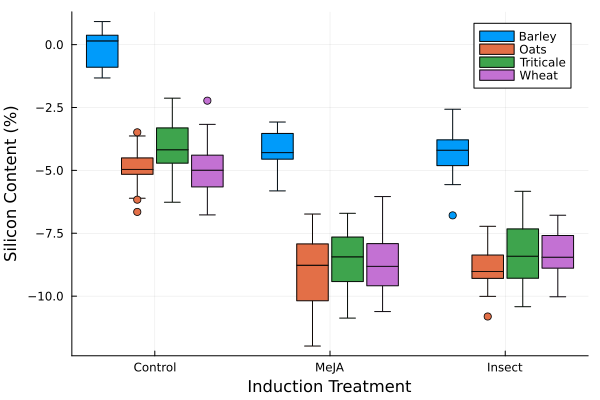
\includegraphics[width = \textwidth]{images/induction_plot.png}
        \centering
        \caption{The effects of crop species and induction treatment on leaf silicon content. Plants were treated either with a 1mM methyl jasmonate spray, or exposure to house crickets \textit{Acheta domesticus}. Leaves were sampled 24 hours after treatment, and were analyzed using XRF.}
\end{figure}

\clearpage



\section{Chapter 2: Genetic drivers of silicon accumulation in a wild ancestor of wheat}

\subsection{Introduction}

With a growing global population, and an increasingly imperiled biosphere, the quest for simultaneous increases in both the output and sustainability of agriculture has spurred development and research into new techniques that can help to feed the world and reduce the negative ecological impacts of large scale agricultural production. Over the past thirty years, research momentum has gathered around plant silicon as a potential tool to effect sustainable increases in crop production, with particular applicability in the cereal crops (\cite{reynolds_silicon_2016,christian_breeding_2022}). Cereal crops are globally important, covering over one-third of the world’s arable land, making up over 50\% of the daily caloric intake for most people (\cite{faostat, rudel_agricultural_2009, awika_major_2011}). Cereals are members of the grass family (Poaceae) and typically have relatively high plant silicon content (\>0.75\% total dry weight) (\cite{reynolds_silicon_2016}). Silicon is highly abundant in many soils globally, and is the second most abundant element in the earth’s crust, behind only oxygen (\cite{ma_functions_2003}). It’s high expression in cereals, high abundance in many soils, and incredible broad spectrum effects on plant vigor and stress tolerance have make it a tantalizing target for improvements in agricultural yield and sustainability. Though plants can complete their life cycle in the absence of silicon, its influence on such a diverse range of plant physiological functions has caused researchers to emphasize its importance relative to other non-essential nutrients. 

Silicon underpins a variety of physiological and developmental strategies that plants use to cope with stress. For biotic stressors, silicon can reduce the damage plants experience from herbivory, increase resistance to fungal pathogens, and improve competitive ability with other organisms (\cite{fauteux_silicon_2005, katz_silicon_2019}). On the abiotic side, silicon supplementation improves plant resistance to soil salinity and heavy metal contamination, improves performance against temperature extremes and high irradiation, and helps plants to cope with drought stress (\cite{cooke_consistent_2016}). In comparing stressed plants grown in the absence or presence of silicon, Si+ plants showed a transcriptome profile similar to unstressed plants (\cite{coskun_controversies_2019}). A current hypothesis explaining the broad-spectrum activity of silicon is presented in Coskun et al. (\citeyear{coskun_controversies_2019}), where the authors suggest that silicon deposited in the apoplast of plant tissues where it modulates biological functions of the plant, and ecological interaction with natural enemies, yielding net positive increases in plant performance [I could be more specific if needed]. Realizing these beneficial effects depends on the plant’s ability to efficiently source silicon from the soil and uptake it in sufficient amounts. Finding ways to improve crops towards increased silicon use efficiency is key to harnessing the benefits that plant silicon can confer. 

Plants gather silicon from the soil solution, using a suite of transporter proteins to pump it into their vascular systems and then transport it throughout the body (\cite{reynolds_silicon_2016}).  Variation in the relative expression of these transporters, as well as differences in the development of the end points for silicon deposition (silica cells), may drive phenotypic variation among individuals. Additionally, individuals may vary in their ability to scavenge silicon from the soil. The soluble form of silicon, silicic acid (SiOH4) has a maximum solubility in water of around 2 mM, though typical soil concentrations range from 0.1 mM to 0.6 mM (\cite{epstein_anomaly_1994}). Soluble silicon in the soil is derived primarily from the weathering of silicate minerals, and secondarily from the remobilization of silicon in decaying plant material (\cite{de_tombeur_silicon_2021-1}). Weathering of silicates releases a host of plant nutrients including Al, Si, Fe, and P (\cite{de_tombeur_silicon_2021-1}). Soil biota can drive weathering, using organic acids and other molecules to complex metal ions off of soil aggregates, making them available for uptake by organisms. Plant roots can release carboxylates and phytosiderophores to weather P and Si out of soil minerals. Along with Si and P mobilization, Mn is often released, and taken up by plants roots. Previous research has used leaf Mn content to proxy for the carboxylate releasing activity of plants (\cite{lambers_leaf_2015}), yet so far I are unaware of any studies looking for quantitative variation among genotypes of leaf Mn. If we could identify regions of the plant genome associated with variation in root weathering activity, we may be able to target this trait in breeding programs that improve nutrient use efficiency, ultimately easing our dependence on external inputs to agricultural fields. 

The use of x-ray fluorescence (XRF) to quantify plant silicon has greatly reduced the costs, danger, and processing time of for studies focussing on this topic (\cite{reidinger_rapid_2012}). XRF works by using low-power x-rays to excite elements in the sample, and measures the resulting emitted light. One of the most exciting features of XRF is the fact that it can analyse multiple elements at once, allowing for broad characterization of the sample for most elements heavier than aluminum. Though XRF is an established technique to measure plant Si, its may also be used to measure other metals of interest, including manganese. In this study I use XRF to quantify variation in Si and Mn content among a diversity panel of a wild ancestor of bread wheat, Aegilops tauschii. This panel has publicly available sequence data, allowing us to perform a genome-wide association sutdy to link Si and Mn variation to genotypic variation, laying the groundwork for future, more targetted, explorations of the genome to identify genetic controls over these traits, and hopefully develop breeding targets to improve plant performance and safeguard yeilds against a destabilizing climate.

\subsection{Methods}

\subsubsection{Plant growing conditions}

For this experiment, I used a the L2 panel of Aegilops tauschii from (\cite{gaurav_population_2021}) grown at three different sites. Two of the sites were outdoors on the University of British Columbia campus, with planting occurring in the fall, while the third site was a glasshouse, where I vernalized seedlings in growth chambers prior to transplanting into the glasshouse environment. For full site details see Supplementary Table S1. Using 151 accessions, I started trays of seedlings in glasshouse or growth chamber environments. At approximately eight weeks after germination, seedlings were transplanted to their field sites. For each environment, I started four replicates of each accession. I planted the plants in a randomized block design, to minimize the effects of soil heterogeneity on our phenotype measurements. Each outdoor block was a 16 m\textsuperscript{2} square, with plants arranged $\sim$35 cm apart. Shortly after transplanting to the field sites, I applied water-soluble fertilizer to improve transplant survival, as well as slow-release fertilizer pellets. Field transplantation took place on the 15th of October 2022 and the 16th of December 2022. For the glasshouse environment, I started seedlings in growth chambers in January 2022. After 12 weeks, I moved the seedlings to vernalization chambers (4ºC, 8:16h light:dark) for eight weeks. I then transplanted these plants into 10cm square pots filled with SunGro potting mix and amended with [amount] of silicic acid (Tixosil 68B, Solvay). Pots were arranged using the same randomized block design, adapted to fit on two flood tables. To ensure a comparable life stage accross environments at time of harvest, these plants grew for three months (mid June – mid September 2022), until they had mature flower heads. 

\subsubsection{Plant harvest and sample preparation}

When the plants had reached maturity, I harvested the entire above-ground portion of each plant. For the outdoor sites, harvest occurred between the 1st and 5th of July 2022, while I harvested the glasshouse plants between the 19th and 21st of September 2022. I placed harvested material in labelled paper bags, and dried it in drying ovens at 60ºC for 48 hours. To harvest leaf material for analysis, I selected stems with flower heads, and removed the three leaves closest to the flowers. Since portions of the plant body have different silicon contents (\cite{dai_genetic_2005}), I chose a consistent set of leaves to minimize introduced variation. I picked leaves until approximately 200mg of dry leaf was collected. I then washed leaves in distilled water to remove any soil residues which might introduce silicon, and re-dried the samples at 60ºC for 48 hours. Dried, clean leaves were then packed into 2 ml microcentrifuge tubes with zircon grinding pellets, flash frozen by immersion in liquid nitrogen, and ground in a tissuelyser ball mill for 30 seconds at 60 Hz. The resulting leaf powder was stored sealed until XRF analysis. 

\subsubsection{Sample analysis}

To analyse the silicon and manganese content of the accessions, I followed the XRF procedure presented in Reidinger et al. (\citedate{reidinger_rapid_2012}). In short, I pressed leaf powder into 13mm diameter pellets at 11 tonnes of pressure and analysed the resulting pellets in an Olympus Vanta p-XRF device mounted in a bench stand. I used a read time of 30s to ensure accurate measurements. To minimize cross-contamination between samples, I wiped clean the pellet press and XRF device after each sample.

\subsubsection{Statistical analysis}

To perfrom the GWAS analysis, I followed the methodology and code published in Gaurav et al. \citedate{gaurav_population_2021}. For brevity, this methodology only describes the steps we took using the data generated from Gaurav et al. \citedate{gaurav_population_2021}. For full details on how they generated the sequence data and prepared the final data sets refer to their manuscript. Prior to the linear regression to assess genetic associations, we first tested our phenotypic data for block effects within sites. For each site, we tested a linear model to see if measured leaf silicon content was significantly associated with block. We tested the model $y \sim Block + Accession$. When we validated that block had a negligible effect ($p>0.1$), we reparameterized leaf silicon measurements at the site level. We converted the raw \%Si to be expressed as the number of standard deviations the sample deviated from the site mean of \%Si. I did this to eliminate a possible confounding effect of inter-site differences that might reduce the power of the GWAS linear regression. 

As per Gaurav et al. \citedate{gaurav_population_2021}, to reduce the computational intensity of my analysis, I prefiltered the total $k$-mer matrix to remove $k$-mers with a low chance of being informative [word choice?]. 

\subsection{Results}

Of the approximately 1700 plants planted, [1300] produced enough leaf material for analysis. Silicon content in \textit{Aegilops tuaschii} ranged from [\textit{value}]\% to [\textit{value}\%]. The various growing environments drove a large amount of variation in silicon content. Overall, my analysis revealed [four] regions of the \textit{Aegilops tauschii} genome that has significant associations with silicon content (Figure \ref{Fig:si_peak_plot}). One of these genomes was on chromosome 4S, near a known gene analogue to \textit{Lsi1}, a silicon transporter protein. My results for manganese content are less clear. I detected no regions that met the threshold for significance, though there were three that had pronounced peaks relative to the average response (Figure \ref{Fig:mn_peak_plot}). Within the plants, silicon and manganese content were correlated ($R^2$ = 0.15, p = 0.049) (Figure 3). 

\subsection{Discussion}

\subsection{Acknowledgements}

\subsection{Data Availability}

\subsection{Tables and Figures}

\begin{figure}[h]
        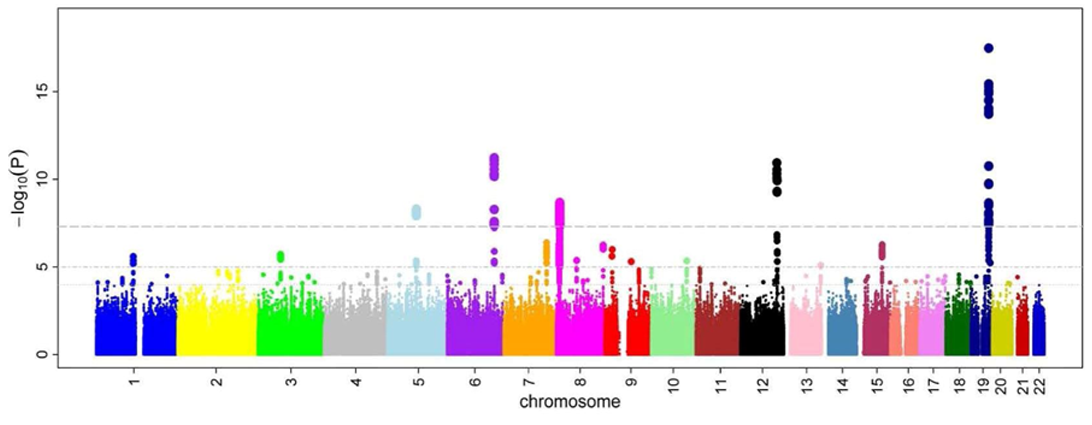
\includegraphics{images/Manhattan_Plot.png}
        \centering
        \caption{This is an example Manhattan Plot from the GWAS output. The real figure will show associations with silicon content}
        \label{Fig:si_peak_plot}
\end{figure}
\begin{figure}[h]
        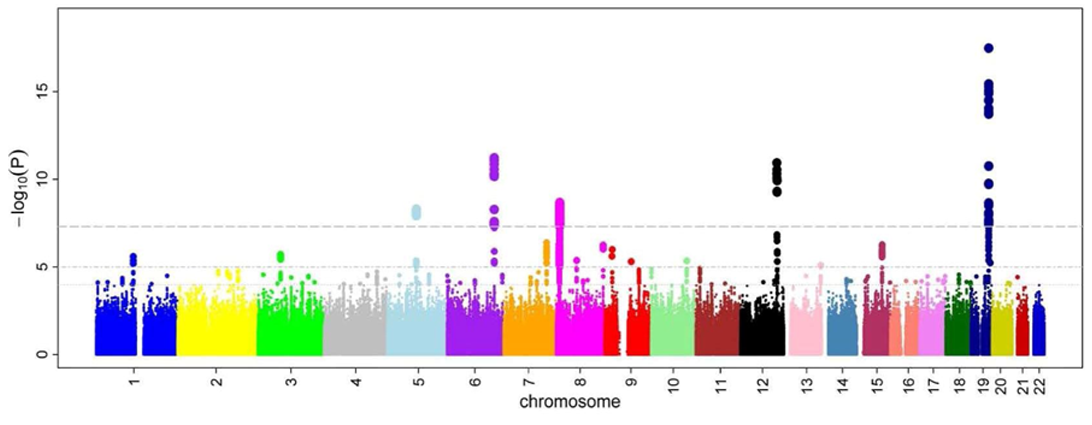
\includegraphics{images/Manhattan_Plot.png}
        \centering
        \caption{This is another Manhattan Plot, this time showing associations with manganese content}
        \label{Fig:mn_peak_plot}
\end{figure}

\begin{figure}[h]
        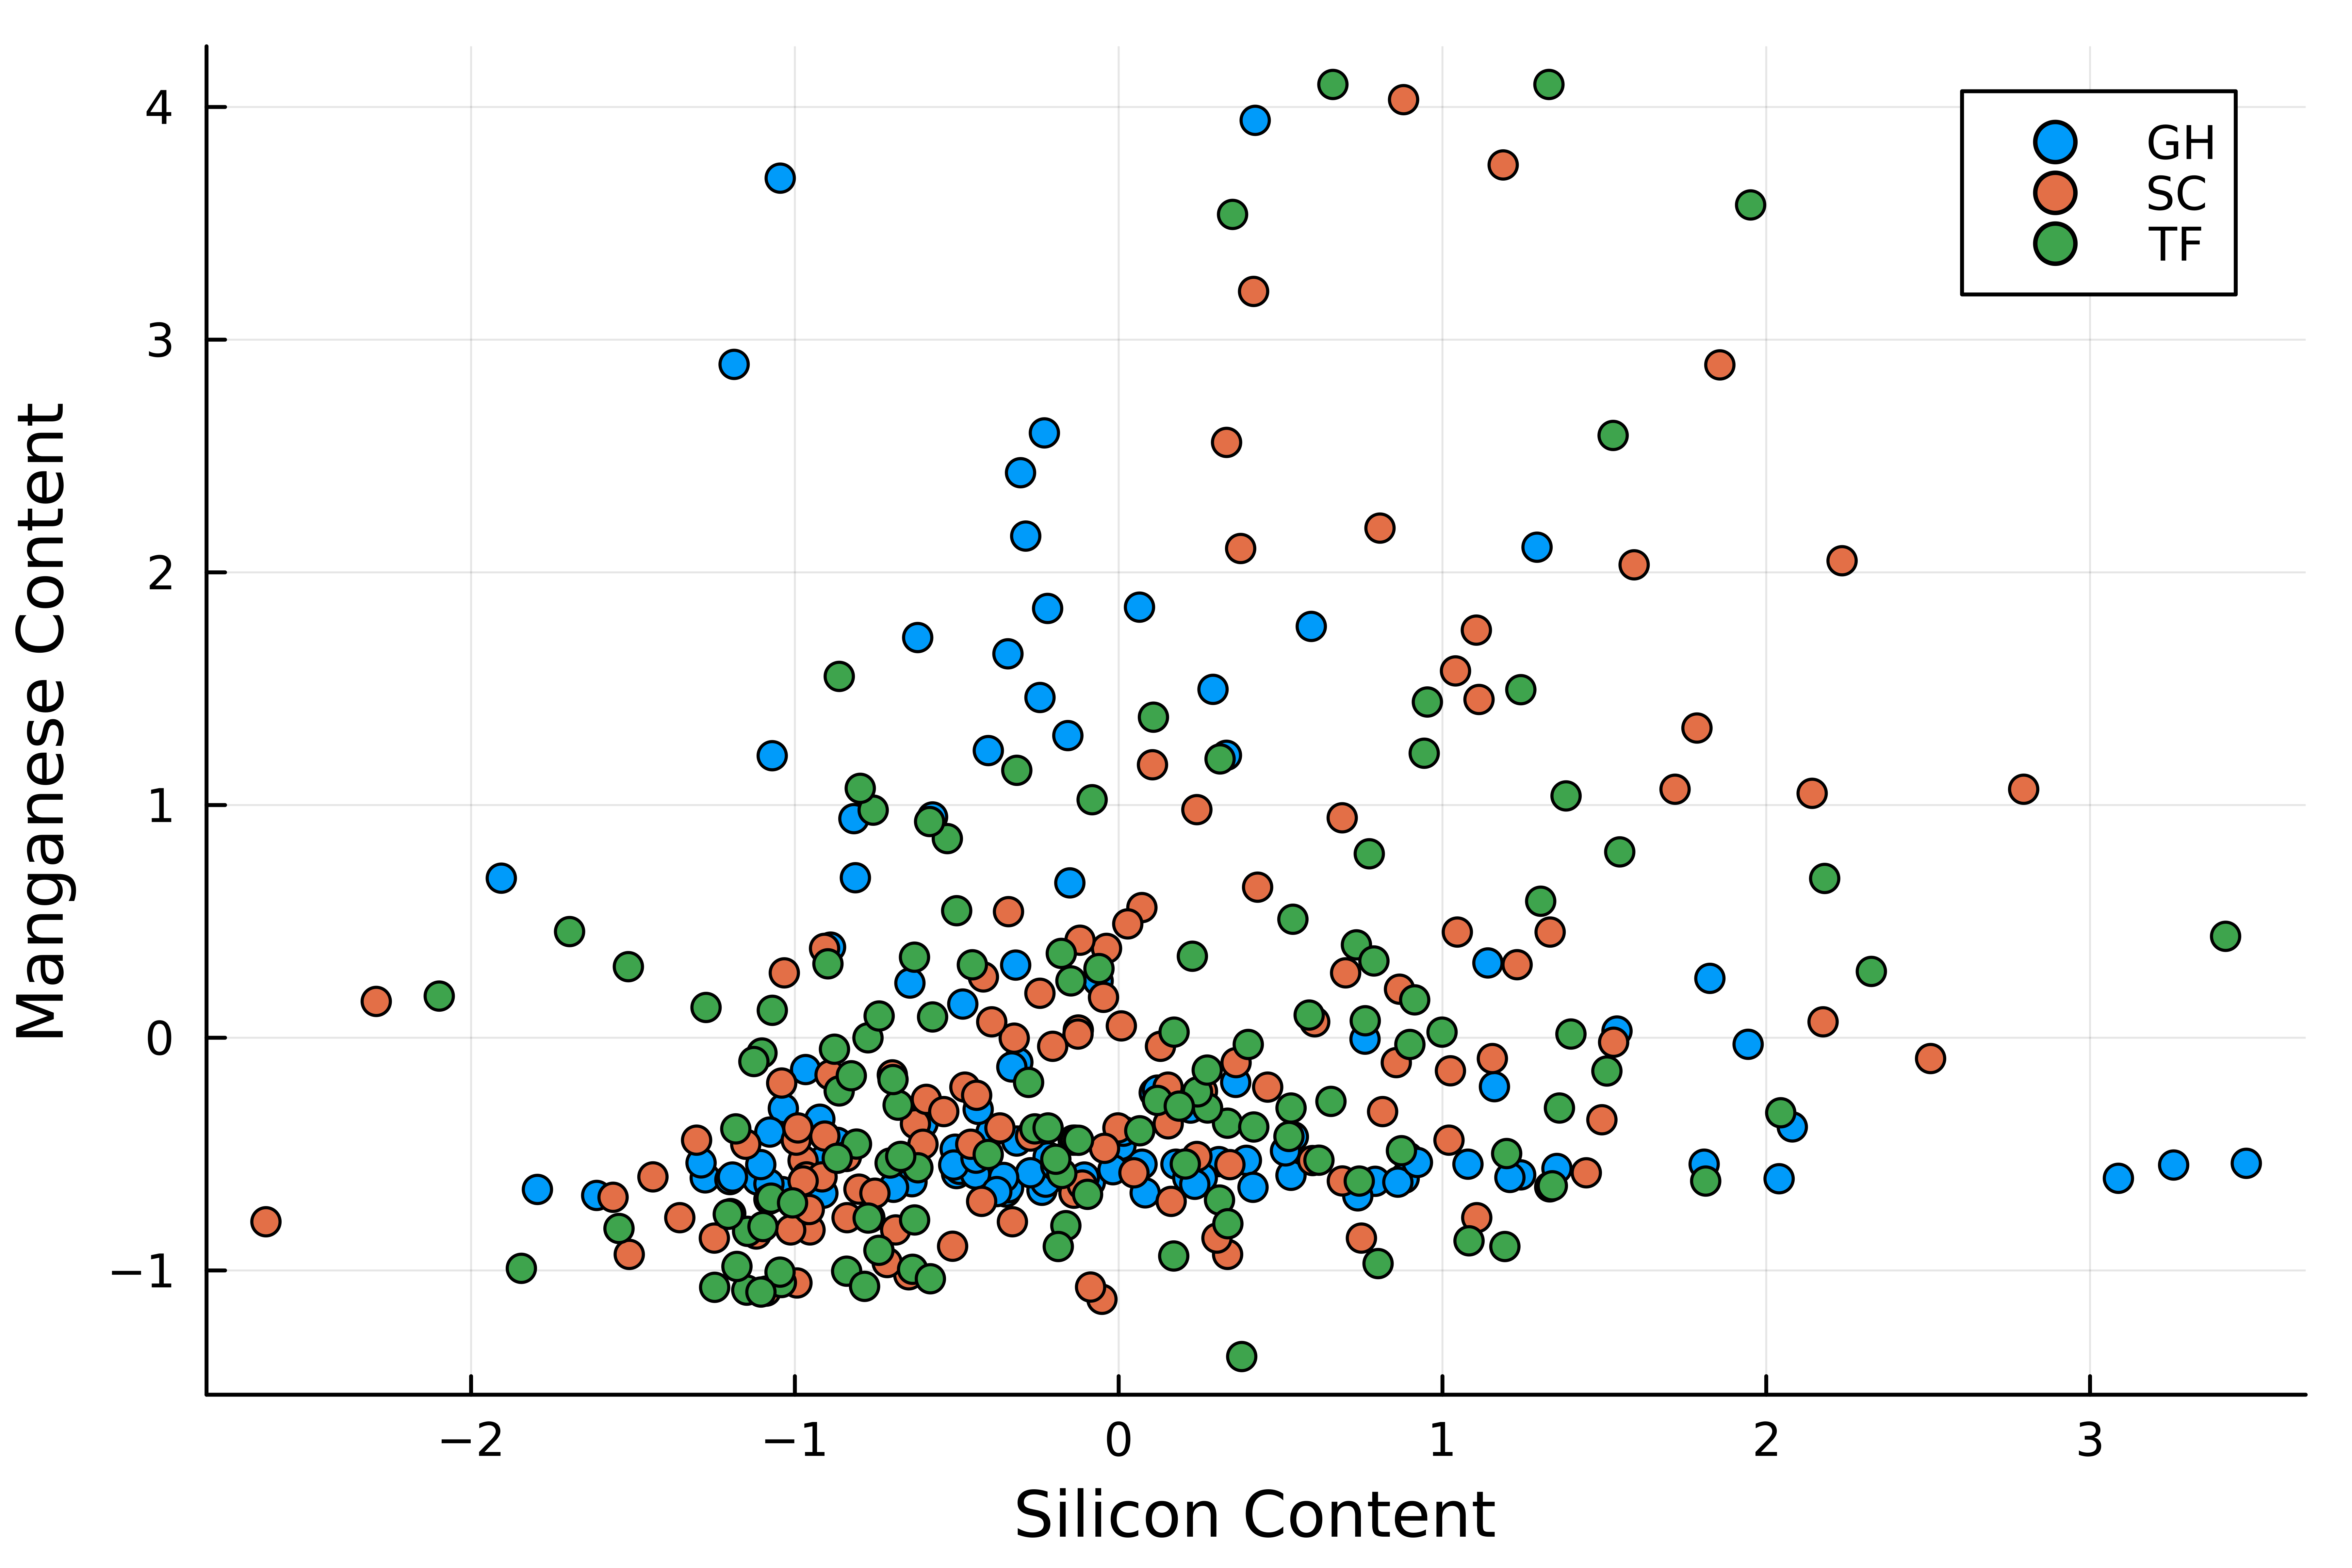
\includegraphics{images/si_mn_regression.png}
        \centering
        \caption{This is the regression comparing Si to Mn content in the leaf tissue}
        \label{Fig:mn_si_regression}
\end{figure}

\clearpage

\section{References}
\printbibliography

\end{document}